\subsection{Dispositivo}

El prototipo, al conectarse a una red eléctrica iniciará el asistente, al igual que dejará corriendo en segundo plano el subproyecto que hemos desarrollado con el fin de poder controlar y monitorizar el propio dispositivo.

\subsubsection{Naturaleza del controlador}

El monitoreo y control remoto de un dispositivo plantea el siguiente dilema: cómo invertir los roles para que un cliente haga de servidor recibiendo información, mientras el servidor hace de cliente mandando a este peticiones.

Para resolver esta adversidad se toma una visión general del proyecto:
\begin{enumerate}
    \item El dispositivo informa cada cierto tiempo de que sigue encendido.
    \item El servidor proporciona una API REST.
\end{enumerate}

Como bien se sabe, los operaciones básicas de una API REST son \textit{GET, POST, PUT y DELETE}, de modo que si se hace una petición \textit{GET} para informar sobre su conexión activa a la red eléctrica, se puede aprovechar por parte del servidor esta llamada para inyectar una acción a realizar en el dispositivo como respuesta a esta llamada.

De este modo el servidor podría manejar el dispositivo, monitorizándolo o pidiendo que haga acciones de manera remota, pudiendo tratarse por ejemplo de una tarea cuya finalidad sea que el asistente inicie una conversación con el usuario final en caso de que haya habido un accidente, de manera que se le pueda ayudar.

Este planteamiento en cuanto a la naturaleza del controlador y su modo de uso parece factible, pero tiene la pega de la usabilidad, ya que si el dispositivo tiene una configuración de mandar su estado cada 24 horas, el control del dispositivo se demoraría demasiado, y aquí entra en juego la siguiente técnica:

Se puede configurar en el propio dispositivo que las 24 horas que pasa entre aviso y aviso se obtengan a partir de un fichero de configuración, que permita la variación de estas 24 horas.
También, en segundo plano, se puede configurar que a ciertas horas, el dispositivo disminuya su periodo de aviso, coincidiendo con unas ciertas horas relativas al horario del admnistrador del sistema, de modo que este pueda mandarle una primera tarea que sea otra reducción del periodo de aviso, por ejemplo a 10 segundos, permitiendo una comunicación síncrona más pareja a una comunicación real, y permitiendo un envío posterior de tareas al dispositivo que se realizarían en un espectro corto de tiempo.

En la figura \ref{fig:prototype-flow} se puede observar el flujo de estados propuesto e implementado en este proyecto con el fin de poder controlar y monitorizar el dispositivo.

\begin{figure}[h!]
    \centering
    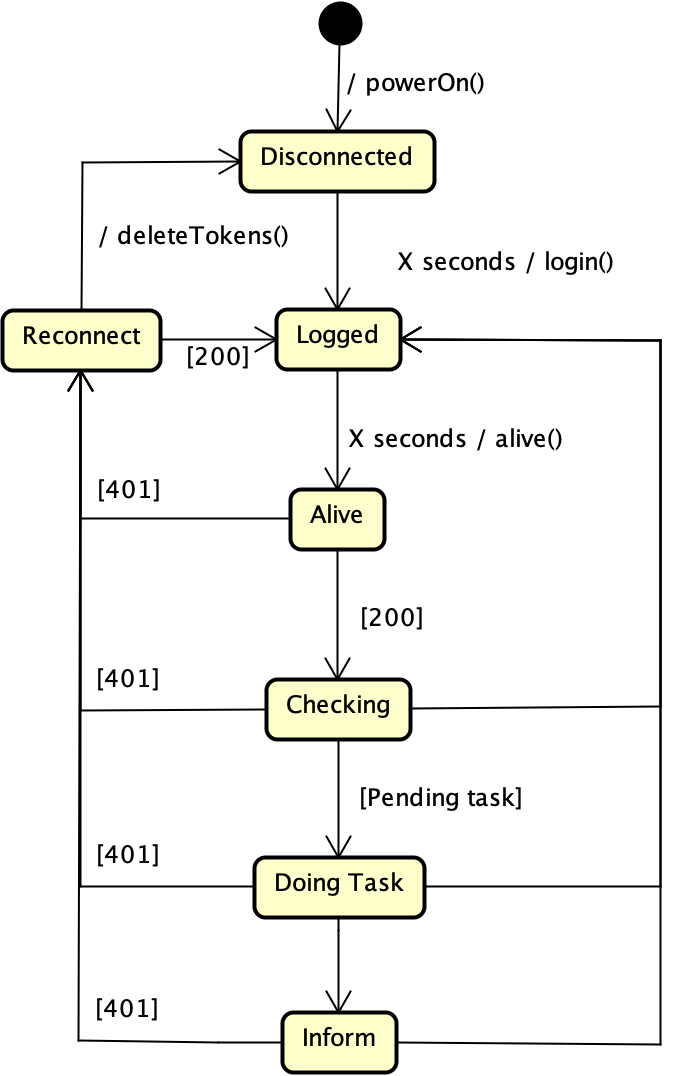
\includegraphics[width=7cm]{./img/state/prototype-flow.png}
    \caption{Flujo de estados del dispositivo}
    \label{fig:prototype-flow}
\end{figure}

\subsubsection{Desarrollo}

ESTRUCTURA DE LO CREADO +++
INICIO AUTOMÁTICO +++
ADICCIÓN DE TAREAS +++

\subsection{BackEnd}


    \subsubsection{Patrones}
    
    \subsubsection{servicios}
    
    \subsubsection{diagrama de clases}
    
    \subsubsection{diagrama entidad relacion}

    \subsubsection{End-Points}
    
\subsection{FrontEnd}

    \subsubsection{Estructura de directorios}
    
    \subsubsection{ (Pre)diseño de interfaz }
    
    \subsubsection{ Lógica }